\documentclass[../main.tex]{subfiles}
%!TEX root = ./appendixBearings.tex
\graphicspath {{../}}

\begin{document}
\section{Bearings} \label{Bearings}
\subsection{Gondola Bearings}

\subsection{Thruster Bearings}

\subsection{Thruster Bearings Press Fit}
The bearing in the Bearing Shaft Support seen in Figure \ref{fig:ShaftLocation} will be mounted using a press fit. The calculations \cite{pressfit} for will need to be used for the bearing as the shaft (bearing into Bearing Bracket). {(Shigley's Machine Design \cite[116]{shigley})}.

\begin{figure}[H]
	\centering
	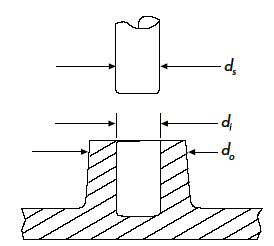
\includegraphics[width=0.5\textwidth]{img/analysis/thruster/pressfit.png}
	\caption{Pressfit Interference Diameters \cite{pressfit}}
	\label{fig:pressfit}
\end{figure}

\begin{equation}
\sigma_r=\frac{\delta}{R[\frac{1}{E_o}\cdot{}(\frac{r_o^2+R^2}{r_o^2-R^2}+v_o)+\frac{1}{E_i}\cdot{}(\frac{R^2+r_i^2}{R^2-r_o^2}+v_i)]}
\end{equation}

\begin{equation}
\sigma_r=\frac{0.1}{20mm[\frac{1}{E_o}\cdot{}(\frac{r_o^2+R^2}{r_o^2-R^2}+v_o)+\frac{1}{E_i}\cdot{}(\frac{R^2+r_i^2}{R^2-r_o^2}+v_i)]}
\end{equation}

\begin{equation}
n=\frac{S_y}{\sigma_a}
\end{equation}
Dimensions were taken as the worst case for the bearing OD. Yield stress for aluminum is 276MPa cite{?????????????}, 316 stainless steel data was taken from cite{???????????}.
\end{equation*}
\end{document}